% THIS IS SIGPROC-SP.TEX - VERSION 3.1
% WORKS WITH V3.2SP OF ACM_PROC_ARTICLE-SP.CLS
% APRIL 2009
%
% It is an example file showing how to use the 'acm_proc_article-sp.cls' V3.2SP
% LaTeX2e document class file for Conference Proceedings submissions.
% ----------------------------------------------------------------------------------------------------------------
% This .tex file (and associated .cls V3.2SP) *DOES NOT* produce:
%       1) The Permission Statement
%       2) The Conference (location) Info information
%       3) The Copyright Line with ACM data
%       4) Page numbering
% ---------------------------------------------------------------------------------------------------------------
% It is an example which *does* use the .bib file (from which the .bbl file
% is produced).
% REMEMBER HOWEVER: After having produced the .bbl file,
% and prior to final submission,
% you need to 'insert'  your .bbl file into your source .tex file so as to provide
% ONE 'self-contained' source file.
%
% Questions regarding SIGS should be sent to
% Adrienne Griscti ---> griscti@acm.org
%
% Questions/suggestions regarding the guidelines, .tex and .cls files, etc. to
% Gerald Murray ---> murray@hq.acm.org
%
% For tracking purposes - this is V3.1SP - APRIL 2009

\documentclass{acm_proc_article-sp}

%\usepackage{url}
\usepackage[hyphens]{url}
\usepackage{textcomp}

\begin{document}

\title{Enabling the Hypermedia Constraint Through HTTP OPTIONS, Link Headers, And The HTTP Vocabulary In RDF}
%
% You need the command \numberofauthors to handle the 'placement
% and alignment' of the authors beneath the title.
%
% For aesthetic reasons, we recommend 'three authors at a time'
% i.e. three 'name/affiliation blocks' be placed beneath the title.
%
% NOTE: You are NOT restricted in how many 'rows' of
% "name/affiliations" may appear. We just ask that you restrict
% the number of 'columns' to three.
%
% Because of the available 'opening page real-estate'
% we ask you to refrain from putting more than six authors
% (two rows with three columns) beneath the article title.
% More than six makes the first-page appear very cluttered indeed.
%
% Use the \alignauthor commands to handle the names
% and affiliations for an 'aesthetic maximum' of six authors.
% Add names, affiliations, addresses for
% the seventh etc. author(s) as the argument for the
% \additionalauthors command.
% These 'additional authors' will be output/set for you
% without further effort on your part as the last section in
% the body of your article BEFORE References or any Appendices.

\numberofauthors{2} %  in this sample file, there are a *total*
% of EIGHT authors. SIX appear on the 'first-page' (for formatting
% reasons) and the remaining two appear in the \additionalauthors section.
%
\author{
% You can go ahead and credit any number of authors here,
% e.g. one 'row of three' or two rows (consisting of one row of three
% and a second row of one, two or three).
%
% The command \alignauthor (no curly braces needed) should
% precede each author name, affiliation/snail-mail address and
% e-mail address. Additionally, tag each line of
% affiliation/address with \affaddr, and tag the
% e-mail address with \email.
%
% 1st. author
\alignauthor Thomas Steiner\\
       \affaddr{Universitat Polit{\'e}cnica de Catalunya}\\
       \affaddr{Department LSI}\\
       \affaddr{08034 Barcelona, Spain}\\
       \email{tsteiner@lsi.upc.edu}
\alignauthor Jan Algermissen\\
       \affaddr{NORD Software Consulting}\\
       \affaddr{Kriemhildstrasse 7}\\
       \affaddr{22559 Hamburg}\\
       \email{info@nordsc.com}
}
% Just remember to make sure that the TOTAL number of authors
% is the number that will appear on the first page PLUS the
% number that will appear in the \additionalauthors section.

\maketitle
\begin{abstract}
In this position paper we present a way how the hypermedia constraint from REST can be enabled using a combination of Link headers, the HTTP OPTIONS method, and the HTTP Vocabulary in RDF. We have implemented our approach in a Web service of ours, and discuss the learnings in the second part of the paper.
\end{abstract}

% A category with the (minimum) three required fields
\category{H.3}{Information Storage and Retrieval}{On-line Information Services}

\terms{Experimentation}

\keywords{REST, Hypermedia Constraint, HATEOAS, HTTP} % NOT required for Proceedings

\section{Introduction}\label{sec:introduction}
In one of his blog posts\footnote{\url{http://roy.gbiv.com/untangled/2008/rest-apis-must-be-hypertext-driven}} Roy T. Fielding complains about the common practice to call any and all HTTP-based interface a REST API. He names a concrete example and writes that it actually "screams RPC" [sic]. Fielding continues that REST APIs must be hypertext driven. He defines\footnote{\url{http://roy.gbiv.com/untangled/2008/rest-apis-must-be-hypertext-driven#comment-718}} \textit{hypertext} (and compares it to the term \textit{hypermedia}) as follows:
\begin{quote}
When I say hypertext, I mean the simultaneous presentation of information and controls such that the information becomes the affordance through which the user (or automaton) obtains choices and selects actions. Hypermedia is just an expansion on what text means to include temporal anchors within a media stream; most researchers have dropped the distinction.

Hypertext does not need to be HTML on a browser. Machines can follow links when they understand the data format and relationship types.
\end{quote}
The essential constraint of REST is the hypermedia constraint, which in the Richardson Maturity Model (see the following section \ref{sec:rmm}) is described as the last step towards the full glory of REST.

\subsection{Richardson Maturity Model (RMM)}\label{sec:rmm}
In the Richardson Maturity Model\footnote{\url{http://martinfowler.com/articles/richardsonMaturityModel.html}} (RMM) Leonard Richardson describes four levels towards true REST. Level zero is about tunneling all data through HTTP with only one HTTP method (usually POST, sometimes also GET) to one and the same endpoint usually using Remote Procedure Calls (RPC) and neglecting any mechanisms of the Web. Level one introduces resources, so rather than talking to just one endpoint, several endpoints are used. Level two switches from just one HTTP method to more adequate methods, oftentimes aligned to the four functions of persistent storage, CREATE, READ, UPDATE, DELETE (CRUD). In addition to different HTTP methods, also different HTTP status codes are used in order to signal failures, conflicts, or success. Finally level three introduces hypermedia controls that give an answer to the question "\textit{where} can one go next" and "\textit{what} can one do next" after each request in form of links. A Web service or API designed along this principles can be autodiscovered by a user agent by simply following her nose.

The authors, however, prefer not to use the RMM because it implies that the three lower levels induce a researched set of properties that imply that there is a known/assessable value in applying only a subset of the REST constraints.

\subsection{On the Hypermedia Constraint}\label{sec:hateoas}
We have cited Fielding's to-the-point definition of \textit{hypermedia}/\textit{hypertext} above. Next, we need to define \textit{application state}. The problem with \textit{application state}, however, is that it is understood differently by different people. We tend to a definition that is explained best with the example of pagination on a search engine results page. Assume each page contained ten results and a link to its direct successor and predecessor. If the current page has a link to page seven and page nine, it can be directly implied that the current page must be page eight, if, and only if, the relation and/or meaning of the links is well-known beforehand. Hence the application is in state eight, without the explicit need to serialize this state somehow. The state machine of an application is not defined by the service, but by the user agent. In other words, the application comes into being by the choices the user agent makes, not by what the service intended.

\section{Present Ways To (Partly) Fulfill the Hypermedia Constraint}\label{sec:currenthateoas}
The hypermedia constraint is enabled by embedding controls (e.g., links, forms) in the representations made available to the client. There is no standard way to represent hypermedia controls, however, there are common practices that we present in the following section (not in any particular order).

\subsection{Atom Syndication Format (RFC4287)}\label{sec:atom}
In the Atom Syndication Format \cite{Atom:Synd} there is the \texttt{atom:link} element that defines a reference from an entry or feed to a Web resource. The structure of the element is as follows:
\begin{verbatim}
atomLink =
  element atom:link {
    atomCommonAttributes,
    attribute href { atomUri },
    attribute rel { atomNCName | atomUri }?,
    attribute type { atomMediaType }?,
    attribute hreflang { atomLanguageTag }?,
    attribute title { text }?,
    attribute length { text }?,
    undefinedContent
  }
\end{verbatim}
The \texttt{@href} attribute has to contain the link's IRI (the response to the question "\textit{where} can one go next"). The response to the question "\textit{what} can one do next" can (not must) be given in the link's \texttt{@rel} attribute. Its value can be a pre-defined value\footnote{The current list of pre-defined link relations is maintained by the IANA at \url{http://www.iana.org/assignments/link-relations/link-relations.xhtml.}}, or an IRI for custom link relations.

\subsection{Google Data Protocol}\label{sec:gdata}
The Google Data Protocol\cite{Google:Data} extends the Atom Publishing Protocol\cite{Atom:Pub} for processing queries, authentication, and batch requests. The Atom Publishing Protocol is an application-level protocol for publishing and editing Web resources. It is based on HTTP transfer of Atom-formatted representations. There are two serializations available: XML and JSON\footnote{\url{http://code.google.com/apis/gdata/docs/json.html}}. The structure of the XML serialization is the same as in \ref{sec:atom}, the structure of the JSON serialization can be seen below:
\begin{verbatim}
"link": [{
  "rel": "...",
  "type": "...",
  "href": "..."
}]
\end{verbatim}
The elements and attributes of the JSON serialization are a straight-forward mapping of the XML serialization. The main advantage of JSON is that it is directly usable in JavaScript.

\subsection{(X)HTML With Or Without Forms}\label{sec:xhtml}
A regular human-readable (X)HTML page can serve as a hypermedia control, too. Contained links and potential surrounding textual can be understood by humans, while machines can process just the links. Forms can give further instructions on the \textit{how} of the next steps. With forms allowed values for parameters, like, e.g., enumerations can be given.

\subsection{Form Technologies}\label{sec:formtechs}
We adopt the term "form technologies" from Leonard Richardson\footnote{\url{http://www.crummy.com/writing/speaking/2008-QCon/act3.html}} to reference a subset of description languages and mechanisms that are commonly criticized as being brittle\footnote{See, e.g., \url{http://bitworking.org/news/193/Do-we-need-WADL} for WADL.}. The goal of such form technologies like the Web Application Description Language (WADL)\footnote{\url{http://www.w3.org/Submission/wadl/}}, RDF Forms\footnote{\url{http://www.markbaker.ca/2003/05/RDF-Forms/}}, or even the Web Services Description Language Version 2.0 (WSDL 2.0)\footnote{\url{http://www.w3.org/TR/wsdl20/}} is to describe the HTTP methods, parameters, and allowed values that are involved during a Web service request. It is to be noted that WSDL 2.0 is a design-time description language, whereas WADL at least \textit{can} be used as a run-time description language. We still decided to mention it because it can be used\footnote{\url{http://www.ibm.com/developerworks/webservices/library/ws-restwsdl/}} to describe REST Web services.

\subsection{Media Types}\label{sec:mediatypes}
Media type give detailed insights into \textit{how} to process a representation. They outline which parts of the representation are hypermedia controls. If media types are defined to be extensible (i.e., in a way that new data can be added without breaking old user agents that did not expect this new data), they can help decouple a service from its implementation. In order to register a new custom media type, a registration template can be submitted for review to the IANA\cite{IANA:Mime}. Specific, i.e., exactly not \texttt{application/json}, \texttt{application/xml} or \texttt{text/xml}) are an essential aspect of achieving self descriptiveness and key for implementing truely RESTful APIs.

\subsection{Link Headers}\label{sec:linkheaders}
In the Web Linking\cite{Link:Headers} proposed standard document Mark Nottingham specifies relation types for Web links and how such links can be used with a Link header field in HTTP. In addition to that the document also defines a registry for link relations in section 6.2.2, therewith updating the relations defined in the Atom Syndication Format. Quoting from \cite{Link:Headers}:
\begin{quote}
The Link entity-header field provides a means for serialising one or more links in HTTP headers.  It is semantically equivalent to the <LINK> element in HTML, as well as the atom:link feed-level element in Atom [RFC4287].
\end{quote}
A concrete example is shown below:
\begin{verbatim}
Link: <http://search.example.org/results/page7>;
    rel="previous"; title="previous results"
Link: <http://search.example.org/results/page9>;
    rel="next"; title="next results"
\end{verbatim}
As outlined in the same example in section \ref{sec:hateoas}, the implication is that the current page is page 8, as the link relations \texttt{previous} and \texttt{next} refer to an ordered series of resources. We want to highlight that link relations are not limited to the set of registered relations, but can be any IRI. If we build the bridge to the world of Linked Data\cite{TimBL:LinkedData} where Tim Berners-Lee defines the four rules for Linked Data, we can see that there, too, URIs play a central role:
\begin{enumerate}
\item Use URIs as names for things.
\item Use HTTP URIs so that people can look up those names.
\item When someone looks up a URI, provide useful information, using the standards (RDF*, SPARQL).
\item Include links to other URIs, so that they can discover more things.
\end{enumerate}
The idea is thus to combine link relations with meaningful Linked Data URIs. How powerful this is can be shown using an example: assume http://example.org/video.webm was a reference to a video file. We can then deliver a Link header along with the video data such as:
\begin{verbatim}
Link: <http://example.org/video.txt>;
    rel="http://dbpedia.org/resource/-
        Transcription_%28linguistics%29";
    title="transcription of the video";
    type="text/plain"
\end{verbatim}

\section{HTTP OPTIONS}\label{sec:httpoptions}
The HTTP OPTIONS is one of the most basic ways to discover a resource. According to section 5.1.1 of the HTTP/1.1 specification\cite{HTTP:Spec} only the methods GET and HEAD must be supported by all general-purpose servers, all other methods are optional. The specification says about OPTIONS:
\begin{quote}
The OPTIONS method represents a request for information about the communication options available on the request/response chain identified by the Request-URI. [\ldots]

A 200 response SHOULD include any header fields that indicate optional features implemented by the server and applicable to that resource (e.g., Allow), possibly including extensions not defined by this specification. The response body, if any, SHOULD also include information about the communication options. The format for such a body is not defined by this specification, but might be defined by future extensions to HTTP. Content negotiation MAY be used to select the appropriate response format.
\end{quote}
HTTP OPTIONS is currently not widely supported. While we have no statistically relevant data, a quick round-check (OPTIONS on the main domain, following potential redirects) of the search engines Yahoo!, Bing, and Google resulted in two 405 Method Not Allowed errors for Bing and Google, whereas Yahoo! delivered the Web site content as if the method was GET. The expected behavior can be seen on our university domain \url{http://www.upc.edu/}, including out-of-HTTP extensions:
\begin{verbatim}
$ curl  -i -X OPTIONS http://www.upc.edu/
HTTP/1.1 200 OK
Allow: GET, HEAD, POST, PUT, DELETE, OPTIONS, TRACE,
    PROPFIND, PROPPATCH, MKCOL, COPY, [...]
Content-Length: 0
\end{verbatim}
We could not find a server that returned a response body, however, using the Node.js\footnote{\url{http://nodejs.org/}} server with the Express framework\footnote{\url{http://github.com/visionmedia/express}} we succeeded in fully controlling both the Allow header and the response body:
\begin{verbatim}
$ curl -i -X OPTIONS http://localhost:3000
HTTP/1.1 200 OK
Content-Type: text/plain; charset=utf-8
Allow: GET, HEAD, OPTIONS
Content-Length: 14

I'M THE BODY!
\end{verbatim}

\section{The HTTP Vocabulary in RDF}\label{sec:httpvocab}
HTTP Vocabulary in RDF\cite{HTTP:RDF} defines a representation of HTTP in Resource Description Framework (RDF)\cite{W3C:RDF}. It is intended to record HTTP or HTTPS request and response messages, including the various headers. Consider the following HTTP request:
\begin{verbatim}
$ curl -i http://dbpedia.org/resource/Barcelona
    -H "Accept: application/rdf+xml"
\end{verbatim}
Modeled in RDF (in Turtle syntax\footnote{\url{http://www.w3.org/TeamSubmission/turtle/}}, prefixes omitted for the sake of brevity) the request looks like this:
\begin{verbatim}
_:req a http:Request ;
  http:httpVersion "1.1" ;
  http:methodName "GET" ;
  http:mthd <http://www.w3.org/2008/http-
      methods#GET> ;
  http:abs_path "/resource/Barcelona" ;
  http:resp _:resp ;
  http:headers (
    [ http:fieldName "Host";
      http:fieldValue "dbpedia.org";
      http:hdrName <http://www.w3.org/2008/-
          http-header#host> ]
    [ http:fieldName "Accept";
      http:fieldValue "application/rdf+xml";
      http:hdrName <http://www.w3.org/2008/-
          http-header#accept> ]
      ) .
\end{verbatim}
Albeit verbous, the RDF triples represent the request in a protocol-compliant way. The response to the request could be modeled in the blank node \texttt{\_:resp}.

\section{Implementation And Lessons Learnt}\label{sec:implementation}
Bringing all the technologies mentioned above together, first, we have Link headers to transparently inject data into a response without touching the body of the HTTP message. Second, we have HTTP OPTIONS as a means of discovering a resource on HTTP level. Third, we have the HTTP Vocabulary in RDF. which allows for HTTP communication to be modeled.

In order to test what can be done with regards to the hypermedia constraint with these technologies, we took an existing Web application of ours\footnote{\url{http://tomayac.com/semwebvid/}}, and converted it into an API with the functionality to automatically annotate YouTube videos in RDF, where the input is a YouTube video ID, and the output an RDF document. In the course of implementing this API, a set of secondary wrapper APIs were implemented as well, one for YouTube video search based on a plaintext query, one for Named Entity Extraction (NEE) based on a text fragment, and one for URI Lookup (UL) based on a plaintext query. See Figure \ref{fig:overview} for an overview of the structure of the services and the link relations between them. We serve the output of these wrapping services with the pseudo media types \texttt{application/prs.atom+json} for YouTube API-based data, with \texttt{application/prs.nee-entity+json} for NEE-based data, and with \texttt{application/prs.ul-entity+json} for UL-based data. The main problem of the Web service are the output constraints of our API: the video annotation service is designed to return RDF in one of its serializations, in consequence the media types are, e.g., \texttt{text/turtle}, or \texttt{application/rdf+xml}. The RDF/XML media type\footnote{\url{http://tools.ietf.org/html/rfc3870}} 

\begin{figure}
 \centering
 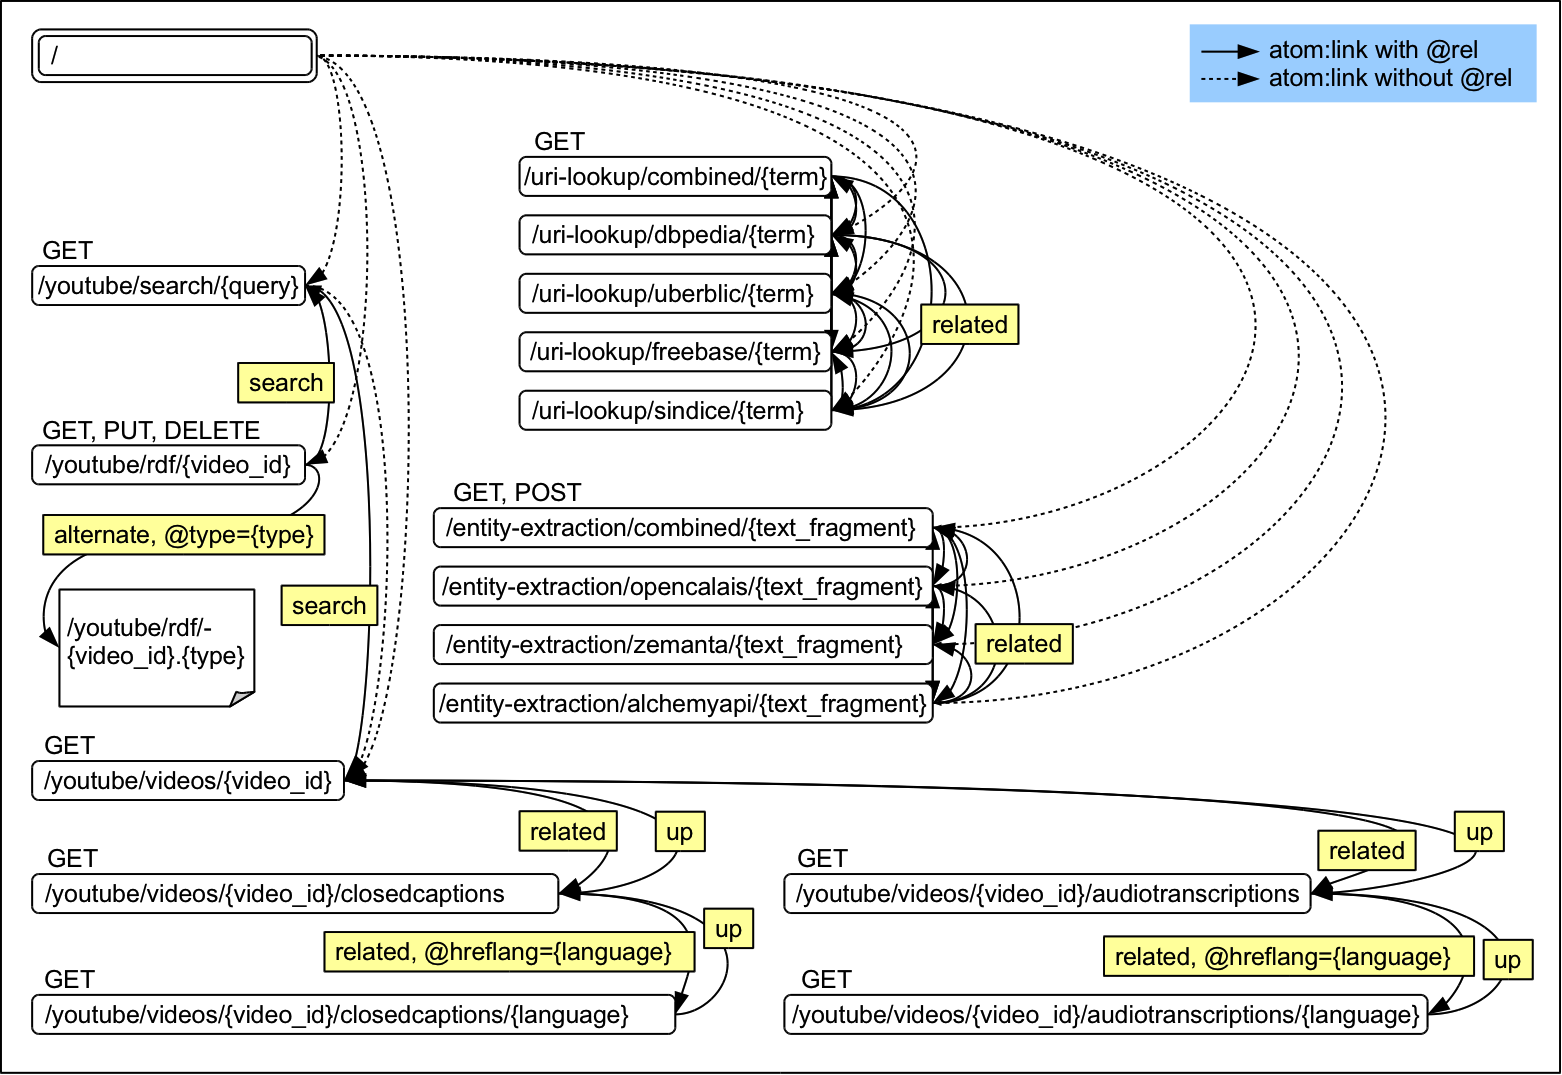
\includegraphics[width=\linewidth]{statemachine.png}
 \caption{Overview of the structure of our Web services with link relations, and allowed HTTP methods.}
 \label{fig:overview}
\end{figure}

\section{Related Work And Conclusion}\label{sec:relatedwork}
\cite{W3C:Blog}

%\end{document}  % This is where a 'short' article might terminate

%ACKNOWLEDGMENTS are optional
\section{Acknowledgments}\label{sec:acknowledgments}
This work is partially funded by the EU FP7 I-SEARCH project (project reference 248296).

%
% The following two commands are all you need in the
% initial runs of your .tex file to
% produce the bibliography for the citations in your paper.
\bibliographystyle{abbrv}
\bibliography{sigproc-sp}  % sigproc.bib is the name of the Bibliography in this case
% You must have a proper ".bib" file
%  and remember to run:
% latex bibtex latex latex
% to resolve all references
%
% ACM needs 'a single self-contained file'!
%
%APPENDICES are optional

%\appendix
%Appendix A
%\balancecolumns
\end{document}
